\section{Data}\label{sec:data}

\textbf{Original Data.} We use the crowdsourced Curlie dataset from Homepage2vec \cite{homepage2vec}, comprising 840 websites. Three annotators assigned top-level categories to each site, and we measured inter-annotator agreement using pairwise Cohen's kappa \cite{cohen-coef}. The mean pairwise Cohen's kappa is $0.2 \pm 0.02$, indicating low agreement. We assign a category label if at least 2 annotators agree, resulting in an average of $2.5$ labels per website. We then scrape and parse HTML content, extracting features such as top-level domain, domain, title, description, keywords, first 50 links, and first 100 sentences.

\begin{table}[!ht]
\centering
\caption{Percentage of websites with each feature accross our datasets.}
\label{tab:feature_information}
\begin{tabular}{lrr}
\toprule
 & Original & Curlie-gpt-10k \\
\midrule
n & 761.00 & 9190.00 \\
tld (\%) & 100.00 & 100.00 \\
domain (\%) & 100.00 & 100.00 \\
tags (\%) & 93.69 & 95.47 \\
titles (\%) & 98.42 & 98.28 \\
descriptions (\%) & 54.93 & 62.95 \\
keywords (\%) & 19.58 & 27.29 \\
links (\%) & 89.88 & 91.62 \\
sentences (\%) & 99.08 & 99.03 \\
\bottomrule
\end{tabular}
\end{table}


\textbf{Curlie-gpt-10k.} We employ the best-performing GPT annotator evaluated against the human annotated original crowdsourced data to annotate \texttt{curlie-gpt-10k}, a dataset with 10k randomly selected websites from Curlie. Following the same preprocessing and feature extraction as the original dataset, Table \ref{tab:feature_information} displays feature percentages across datasets. As the figure clearly indicates, the most useful features according to the homepage2vec \cite{homepage2vec} descriptions and keywords are missing in around 55 \% and 75 \% of cases, respectively. 

\begin{figure}[!ht]
    \centering
    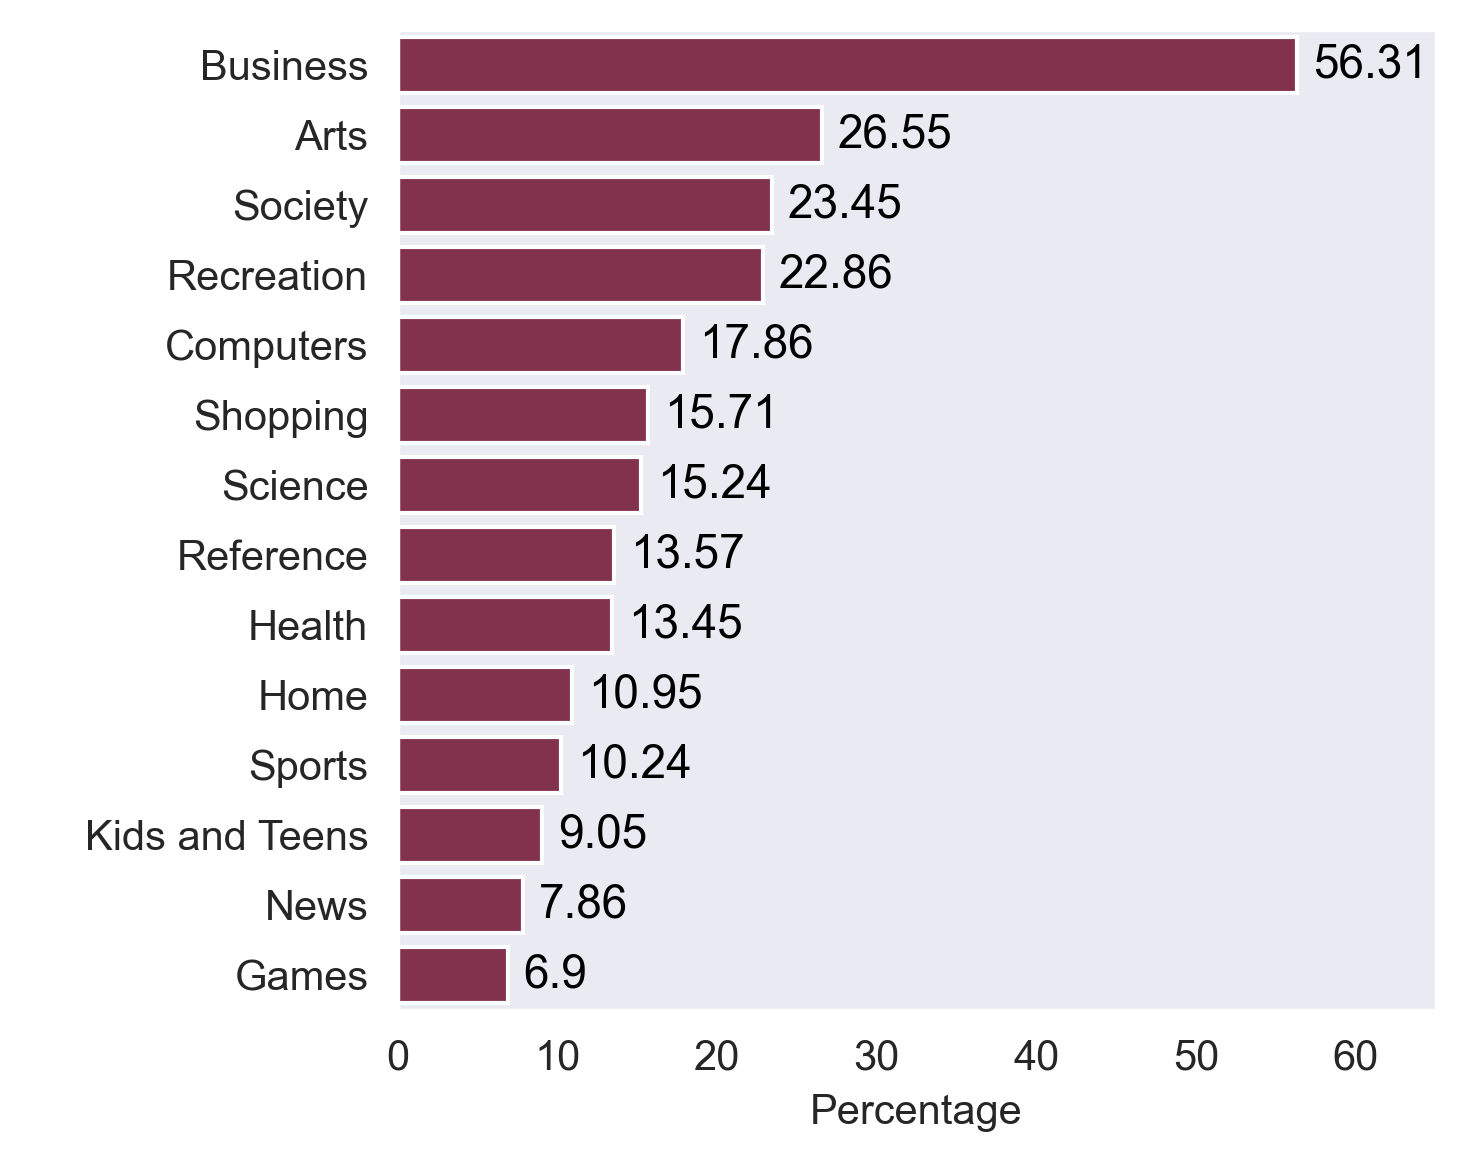
\includegraphics[width=1\columnwidth]{figures/category_distribution.png}
    \caption{Class distribution of the original dataset.}
    \label{fig:class_distribution}
\end{figure}

Figure \ref{fig:class_distribution} illustrates the class distribution of the original dataset. It is imbalanced, with most websites falling into the \textit{Business} category, followed by \textit{Arts} and \textit{Society}. This imbalance, identified in Homepage2vec, negatively impacted model performance on minority classes. We will address this issue in our Methods section.